\documentclass[a4paper, 14pt]{extarticle}

% file's preambule

% Если вы работаете не в XeLaTeX, то сами разбирайтесь =)

% connect packages
%%%%%%%%%%%%%%%%%%%%%%%%%%%%%%%%%%%%%%%%%%%%%%%%%%%%%%%%%%%%%%%%%%%%%%
%\usepackage[T2A]{fontenc}                   %!? закрепляет внутреннюю кодировку LaTeX
%\usepackage[utf8]{inputenc}                 %!  закрепляет кодировку utf8
\usepackage{fontspec}                        % Шрифты
\usepackage{indentfirst}                    %   добавить indent перед первым параграфом
\setlength{\parindent}{1.27cm}
\usepackage{polyglossia}                     % Русский язык
\setdefaultlanguage{russian}
\setmainfont[Ligatures=TeX]{Times New Roman}
\newfontfamily\cyrillicfont{Times New Roman}[Script=Cyrillic]
%\usepackage[english,russian]{babel}         %!  подключает русский и английский
\usepackage{amsmath}                        %!  |
\usepackage{amssymb,textcomp, esvect,esint} %!  |важно для формул 
\usepackage{geometry}                       %!  отступ от граней
\geometry{verbose,a4paper,tmargin=2cm,bmargin=2cm,lmargin=3cm,rmargin=1cm}
\usepackage{amsfonts}                       %!  математические шрифты
\usepackage{amsthm}                         %!  newtheorem и их сквозная нумерация
\usepackage{graphicx}                       %?  графическое изменение текста
\usepackage{soulutf8}% Поддержка переносоустойчивых подчёркиваний и зачёркиваний
\usepackage{enumitem}                       %!  задание макета перечня.
%\usepackage[unicode, pdftex]{hyperref}      %!  оглавление для панели навигации по PDF-документу + гиперссылки
\usepackage{setspace}                       % Межстроковые интервалы
\onehalfspacing
\usepackage{booktabs}                       %!  добавляет книжные линии в таблицы
%\usepackage{hypcap}                         %?  адресация на картинку, а не на подпись к ней
\usepackage{abraces}                        %?  фигурные скобки сверху или снизу текста
\usepackage{caption}                        %-  позволяет корректировать caption 
\DeclareCaptionLabelSeparator{dash}{ - }
\captionsetup[table]{labelformat=simple, labelsep=dash, justification=raggedleft,
singlelinecheck=off}
\captionsetup[figure]{labelformat=simple, labelsep=dash}
\usepackage{multirow}                       %   объединение ячеек в таблицах
\usepackage{longtable}
\usepackage{pifont}                         %!  нужен для крестика
\usepackage{cancel}                         %!  аутентичное перечеркивание текста
\usepackage{ulem}                           %!  перечеркивание текста
\usepackage{tikz}                           %!  высокоуровневые рисунки (кружочек)
\usepackage{titling}                        %-  автоматическое заглавие 
\usepackage{titlesec}  % нормальные заголовки секций
\titleformat{\section}
{\normalfont\large\bfseries\filcenter}{}{1em}{}
\titleformat{\subsection}
  {\normalfont\normalsize\bfseries}{\thesubsection.}{5pt}{}
\titleformat{\subsubsection}
  {\normalfont\normalsize\bfseries}{\thesubsubsection.}{5pt}{}
\titleformat{\paragraph}
  {\normalfont\normalsize\bfseries}{\theparagraph}{5pt}{}

\usepackage{ragged2e} % Для выравнивания текста по ширине
\justifying

%\renewcommand{\thesubsubsection}{\alph{subsubsection}}
\usepackage{blindtext}                      %-  слепой текст
\usepackage{fancyhdr}                       %   добавить верхний и нижний колонтитул
\usepackage{mathptmx}

\usepackage{import}                         %|
\usepackage{xifthen}                        %|
\usepackage{pdfpages}                       %|
%\usepackage{transparent}                    %| вставка ink figures
\usepackage{rotating}
\usepackage{array} % Картиночки в таблицы
%%%%%%%% Алгоритмы
\usepackage{float}
\usepackage{algorithm}
\usepackage{algpseudocode}
%%%%%%%%%%%%%%%

\usepackage{listings} % Для языков программирования 
\usepackage{xcolor}
\lstset {
    language=C++,
    backgroundcolor=\color{black!5}, % set backgroundcolor
    basicstyle=\footnotesize,% basic font setting
}

\usepackage{lmodern}

\colorlet{comment}{green!50!black}
\colorlet{cppcomment}{teal}
\colorlet{symb}{blue!50!black}
\colorlet{number}{violet}

\newcommand*{\textcolorsymb}{\textcolor{symb}}

\definecolor{backcolour}{rgb}{0.95,0.95,0.92}
\definecolor{black_red}{rgb}{0.54, 0, 0}

\lstdefinestyle{cpp}{%
  language=C++,
  columns=flexible,
  basewidth=.5em,  
  tabsize=2,
  basicstyle=\footnotesize,
  backgroundcolor=\color{backcolour},
  showspaces=false,
  showstringspaces=false,
  commentstyle={\itshape\color{comment}\let\textcolorsymb\relax},
  keywordstyle=\bfseries\color{black_red},
  morecomment={[l][\itshape\color{cppcomment}\let\textcolorsymb\relax]//},
  literate=%
    {\{}{\textcolorsymb{\{}}1
    {\}}{\textcolorsymb{\}}}1
    {(}{\textcolorsymb{(}}1
    {)}{\textcolorsymb{)}}1
    {;}{\textcolorsymb{;}}1
    {=}{\textcolorsymb{=}}1
    {<}{\textcolorsymb{<}}1
    {>}{\textcolorsymb{>}}1
    {!}{\textcolorsymb{!}}1
    {\&}{\textcolorsymb{\&}}1 
    {|}{\textcolorsymb{|}}1
    {?}{\textcolorsymb{?}}1
    {:}{\textcolorsymb{:}}1
    {+}{\textcolorsymb{+}}1
    {-}{\textcolorsymb{-}}1
    {,}{\textcolorsymb{,}}1
    {\%}{\textcolorsymb{\%}}1
    {\^}{\textcolorsymb{\textasciicircum}}1
    {~}{\textcolorsymb{\textasciitilde}}1
    %% {/}{\textcolorsymb{/}}1
    %% {*}{\textcolorsymb{*}}1
    % 2 (optionally)
    {==}{\textcolorsymb{==}}2
    {>=}{\textcolorsymb{=>}}2
    {<=}{\textcolorsymb{<=}}2
    {!=}{\textcolorsymb{!=}}2
    {+=}{\textcolorsymb{+=}}2
    {-=}{\textcolorsymb{-=}}2
    {*=}{\textcolorsymb{*=}}2
    {/=}{\textcolorsymb{/=}}2
    {\%=}{\textcolorsymb{\%=}}2
    {\&\&}{\textcolorsymb{\&\&}}2
    {||}{\textcolorsymb{||}}2
    {++}{\textcolorsymb{++}}2
    {--}{\textcolorsymb{--}}2
    {>>}{\textcolorsymb{>\kern0pt>}}2
    {<<}{\textcolorsymb{<\kern0pt<}}2
    {::}{\textcolorsymb{::}}2
    % 3 (optionally)
    {>>=}{\textcolorsymb{>\kern0pt>=}}3
    {<<=}{\textcolorsymb{<\kern0pt<=}}3
    % Remove byte order mark
    {^^ef^^bb^^bf}{}0
}
\lstnewenvironment{cpp}{\lstset{style=cpp}}{}
\lstset{style=cpp}
  


%%%%%%%%%%%%%%%%%%%%%%%%%%%%%%%%%%%%%%%%%%%%%%%%%%%%%%%%%%%%%%%%%%%%%%


%%%%%%%%%%%%%%%%%% ВСТАВКА РИСУНКО ИЗ INKSCAPE %%%%%%%%%%%%%%%%%%%%%%%
\newcommand{\incfig}[1]{%
    \def\svgwidth{\columnwidth}
    \import{./figures/}{#1.pdf_tex}
}

%%%%%%%%%%%%%%%%%%%%%%%%%%%%%%%%%%%%%%%%%%%%%%%%%%%%%%%%%%%%%%%%%%%%%%


\newenvironment{itemize*}
{
    \begin{itemize}
        \setlength{\itemsep}{1pt}
        \setlength{\parskip}{1pt}}
    {\end{itemize}
}

\newenvironment{enumerate*}
{
    \begin{enumerate}
        \setlength{\itemsep}{1pt}
        \setlength{\parskip}{1pt}}
    {\end{enumerate}
}

%%%%%%%%%%%%%%%%%%%%%%%%%%%%%%%%%%%%%%%%%%%%%%%%%%%%%%%%%%%%%%%%%%%%%%


\begin{document}

\includepdf{titul_eighth}
\newpage
\tableofcontents
\newpage
\section{Задание 1}
\textit{Вариант 2.}

\subsection{Упражнение 1}
Условие: Провести преобразование инфиксной записи выражения в
постфиксную нотацию, расписывая процесс по шагам
S=x-(y*a/b-(z+d*e)+c)/f

Алгоритм преобразования отображен в таблице \ref{tab:first_ex}.

\begin{longtable}[htpb]{|c|c|c|c|c|}
  \caption{Упражнение 1 задания 1}
  \label{tab:first_ex}
  \\
    \hline
    Токен & Действие & Вывод & Стек & Комментарий
    \\ \hline
    x & Добавить токен в вывод & x & &
    \\ \hline
    - & Положить токен в стек & x & - &
    \\ \hline
    ( & Положить токен в стек & x & (- &
    \\ \hline
    y & Добавить токен в вывод & xy & (- &
    \\ \hline
    * & Положить токен в стек & xy & *(- &
    \\ \hline
    a & Добавить токен в вывод & xya & *(- &
    \\ \hline
    / & Положить токен в стек & xya & /*(- &
    \\ \hline
    b & Добавить токен в вывод & xyab & /*(- &
    \\ \hline
    \multirow{2}*{-} & \parbox[m]{5cm}{\centering Добавлять токен в вывод
    пока он не равен '('} & xyab/* & (- &
    \\ \cline{2-5}
                     & \parbox[m]{5cm}{\centering Положить токен в стек}& xyab/* & -(- &
    \\ \hline
    ( & Положить токен в стек & xyab/* & (-(- &
    \\ \hline
    z & Добавить токен в вывод & xyab/*z & (-(- &
    \\ \hline
    + & Положить токен в стек & xyab/*z & +(-(- &
    \\ \hline
    d & Добавить токен в вывод & xyab/*zd & +(-(- &
    \\ \hline
    * & Положить токен в стек & xyab/*zd & *+(-(- &
    \\ \hline
    e & Добавить токен в вывод & xyab/*zde & *+(-(- &
    \\ \hline
    \multirow{2}*{)} & \parbox[m]{5cm}{\centering Добавить токен в вывод из стека}& xyab/*zde*+ &(-(-
                     & \parbox[m]{4cm}{\centering Повторять пока не найдена (}
    \\ \cline{2-5}
                     & Удалить из стека токен & xyab/*zde*+ & -(- 
                     & Убираем скобки
    \\ \hline
    + & Положить токен в стек & xyab/*zde*+ & +-(- &
    \\ \hline
    c & Добавить токен в вывод & xyab/*zde*+c & +-(- &
    \\ \hline
    \multirow{2}*{)} & \parbox[m]{5cm}{\centering Добавить токен в вывод из стека}& xyab/*zde*+c+- &(-
                     & \parbox[m]{4cm}{\centering Повторять пока не найдена (}
    \\ \cline{2-5}
                     & Удалить из стека токен  & xyab/*zde*+c+- & - 
                     & Убираем скобки
    \\ \hline
    / & Положить токен в стек & xyab/*zde*+c+- & /- &
    \\ \hline
    f & Добавить токен в вывод & xyab/*zde*+c+-f & /- &
    \\ \hline
    Конец & \parbox[m]{5cm}{\centering Добавляем оставшиеся токены из стека} & xyab/*zde*+c+-f/- & &
    \\ \hline
\end{longtable}

Результат: xyab/*zde*+c+-f/-.
\subsection{Упражнение 2}
Представить постфиксную нотацию выражний:
\begin{enumerate}
  \item (((a+b*c)/d+(x*y-z/k)+m)*n)
  \item a+b/c+d+e-f/m*k
\end{enumerate}

Алгоритм преобразования показан на таблицах \ref{tab:second1_ex} и 
\ref{tab:second2_ex}.
\begin{longtable}[htpb]{|p{3cm}|p{5cm}|p{3cm}|}
  \caption{Упражнение 2.1 задания 1}
  \label{tab:second1_ex}
  \\
    \hline
    Токен & Вывод & Стек
    \\ \hline
    ( & & (
    \\ \hline
    ( & & ((
    \\ \hline
    ( & & (((
    \\ \hline
    a & a & (((
    \\ \hline
    + & a & +(((
    \\ \hline
    b & ab & +(((
    \\ \hline
    * & ab & *+(((
    \\ \hline
    c & abc & *+(((
    \\ \hline
    ) & abc*+ & ((
    \\ \hline
    / & abc*+ & /((
    \\ \hline
    d & abc*+d & /((
    \\ \hline
    + & abc*+d/ & +((
    \\ \hline
    ( & abc*+d/ & (+((
    \\ \hline
    x & abc*+d/x & (+((
    \\ \hline
    * & abc*+d/x & *(+((
    \\ \hline
    y & abc*+d/xy & *(+((
    \\ \hline
    - & abc*+d/xy* & -(+((
    \\ \hline
    z & abc*+d/xy*z & -(+((
    \\ \hline
    / & abc*+d/xy*z & /-(+((
    \\ \hline
    k & abc*+d/xy*zk & /-(+((
    \\ \hline
    ) & abc*+d/xy*zk/- & +((
    \\ \hline
    + & abc*+d/xy*zk/- & ++((
    \\ \hline
    m & abc*+d/xy*zk/-m & ++((
    \\ \hline
    ) & abc*+d/xy*zk/-m++ & (
    \\ \hline
    * & abc*+d/xy*zk/-m++ & *(
    \\ \hline
    n & abc*+d/xy*zk/-m++n & *(
    \\ \hline
    ) & abc*+d/xy*zk/-m++n*& 
    \\ \hline
\end{longtable}
Результат: abc*+d/xy*zk/-m++n*.

\begin{longtable}[htpb]{|p{3cm}|p{5cm}|p{3cm}|}
  \caption{Упражнение 2.2 задания 1}
  \label{tab:second2_ex}
  \\
    \hline
    Токен & Вывод & Стек
    \\ \hline
    a & a & 
    \\ \hline
    + & a & +
    \\ \hline
    b & ab & +
    \\ \hline
    / & ab & /+
    \\ \hline
    c & abc & /+
    \\ \hline
    + & abc/ & ++
    \\ \hline
    d & abc/d & ++
    \\ \hline
    + & abc/d & +++
    \\ \hline
    e & abc/de & +++
    \\ \hline
    - & abc/de & -+++
    \\ \hline
    f & abc/def & -+++
    \\ \hline
    / & abc/def & /-+++
    \\ \hline
    m & abc/defm & /-+++
    \\ \hline
    * & abc/defm & */-+++
    \\ \hline
    k & abc/defmk & */-+++
    \\ \hline
    Конец & abc/defmk*/-+++ &
    \\ \hline
    \end{longtable}
Результат: abc/defmk*/-+++.
\subsection{Упражнение 3}
Представить префиксную нотацию выражний:
\begin{enumerate}
  \item (((a+b*c)/d+(x*y-z/k)+m)*n)
  \item a+b/c+d+e-f/m*k
\end{enumerate}
Для преобразования в префиксную форму перевернем строки,
а затем результат, полученный в результате преобразований,
еще раз перевернем, что даст нам необходимый результат:
\begin{enumerate}
  \item (n*(m+(k/z-y*x)+d/(c*b+a)))
  \item k*m/f-e+d+c/b+a
\end{enumerate}

Алгоритм преобразования показан на таблицах \ref{tab:third1_ex} и 
\ref{tab:third2_ex}.
\begin{longtable}[htpb]{|p{3cm}|p{5cm}|p{3cm}|}
  \caption{Упражнение 3.1 задания 1}
  \label{tab:third1_ex}
  \\
    \hline
    Токен & Вывод & Стек
    \\ \hline
    ( & & (
    \\ \hline
    n & n & (
    \\ \hline
    * & n & *(
    \\ \hline
    ( & n & (*(
    \\ \hline
    m & nm & (*(
    \\ \hline
    + & nm & +(*(
    \\ \hline
    ( & nm & (+(*(
    \\ \hline
    k & nmk & (+(*(
    \\ \hline
    / & nmk & /(+(*(
    \\ \hline
    z & nmkz & /(+(*(
    \\ \hline
    - & nmkz/ & -(+(*(
    \\ \hline
    y & nmkz/y & -(+(*(
    \\ \hline
    * & nmkz/y & *-(+(*(
    \\ \hline
    x & nmkz/yx & *-(+(*(
    \\ \hline
    ) & nmkz/yx*- & +(*(
    \\ \hline
    + & nmkz/yx*- & ++(*(
    \\ \hline
    d & nmkz/yx*-d & ++(*(
    \\ \hline
    / & nmkz/yx*-d & /++(*(
    \\ \hline
    ( & nmkz/yx*-d & (/++(*(
    \\ \hline
    c & nmkz/yx*-dc & (/++(*(
    \\ \hline
    * & nmkz/yx*-dc & *(/++(*(
    \\ \hline
    b & nmkz/yx*-dcb & *(/++(*(
    \\ \hline
    + & nmkz/yx*-dcb* & +(/++(*(
    \\ \hline
    a & nmkz/yx*-dcb*a & +(/++(*(
    \\ \hline
    ) & nmkz/yx*-dcb*a+ & /++(*(
    \\ \hline
    ) & nmkz/yx*-dcb*a+/++ & *(
    \\ \hline
    ) & nmkz/yx*-dcb*a+/++* &
    \\ \hline
    \end{longtable}
Результат: *++/+a*bcd-*xy/zkmn.

\begin{longtable}[htpb]{|p{3cm}|p{5cm}|p{3cm}|}
  \caption{Упражнение 3.2 задания 1}
  \label{tab:third2_ex}
  \\
    \hline
    Токен & Вывод & Стек
    \\ \hline
    k & k & 
    \\ \hline
    * & k & *
    \\ \hline
    m & km & *
    \\ \hline
    / & km & /*
    \\ \hline
    f & kmf & /*
    \\ \hline
    - & kmf/* & -
    \\ \hline
    e & kmf/*e & -
    \\ \hline
    + & kmf/*e & +-
    \\ \hline
    d & kmf/*ed & +-
    \\ \hline
    + & kmf/*ed & ++-
    \\ \hline
    c & kmf/*edc & ++-
    \\ \hline
    / & kmf/*edc & /++-
    \\ \hline
    b & kmf/*edcb & /++-
    \\ \hline
    + & kmf/*edcb/ & +++-
    \\ \hline
    a & kmf/*edcb/a & +++-
    \\ \hline
    Конец & kmf/*edcb/a+++- &
    \\ \hline
\end{longtable}
Результат: -+++a/bcde*/fmk.
\subsection{Упражнение 4}
Провести вычисление значения выражения в префиксной форме,
расписывая процесс по шагам
+7/-9 3*2 5

Перевернем запись для нашего вычисления: 5 2*3 9-/7+
Процесс вычисления значения представленного выражения с
использованием стека приведен в таблице \ref{tab:fourth_ex}.
\begin{longtable}[htpb]{|p{3cm}|p{5cm}|p{3cm}|}
  \caption{Упражнение 4 задания 1}
  \label{tab:fourth_ex}
  \\
    \hline
    Токен & Стек & Результат
    \\ \hline
    5 & 5 &
    \\ \hline
    2 & 2 5 &
    \\ \hline
    * & & 2 * 5 = 10
    \\ \hline
    3 & 3 10 &
    \\ \hline
    9 & 9 3 10 & 
    \\ \hline
    - & 10 & 9 - 3 = 6
    \\ \hline
    / &  & 6 / 10 = 0
    \\ \hline
    7 & 7 0 &
    \\ \hline
    + &  & 7 + 0 = 7
    \\ \hline
    Конец & 7 & 
    \\ \hline
\end{longtable}
Результат = 7.

\section{Задание 2}
\subsection{Задача 1}
\subsubsection{Условие задачи}
Реализовать операции над очередью: втолкнуть элемент в очередь,
вытолкнуть элемент из очереди, вернуть значение элемента в вершине
очереди, сделать очередь пустой, определить пуста ли очередь.
Рассмотреть два варианта реализации очереди: на массиве (или строке);
на однонаправленном списке.
\begin{itemize}
 \item Создать класс или просто заголовочный файл с функциями.
 \item Применить операции для вычисления значения выражения п.1.4 варианта 2.
 \end{itemize}
\subsubsection{Постановка задачи}
Выбрать структуру данных для реализации очереди и описать функции
работы с очередью, реализовать функцию вычисления значения выражения,
записанного в префиксной форме.
\subsubsection{Выбор структуры данных}
В качестве структуры данных для стека рациональней использовать
односвязный список с указателями на начало и конец списка т.к. данная структура имеет
наименьшую асимптотическую сложность вставки и удаления элемента - $O(1)$.
% Но прикол в том, что здесь тратится больше памяти на работу,
% поэтому оценивая неалгоритмически массив может быть намного выгодней,
% имея амортизированную О(1) вставку и удаление в среднем случае.
Информационной частью линейного списка является строковое значение (в общем случае - шаблон),
хранящее токены из заданного выражения и результаты промежуточных подсчетов.
\subsubsection{Код реализации структуры данных}
\lstinputlisting[firstline=1, lastline=78]{code/parsing.cpp}
\subsubsection{Код вычисления выражений}
\lstinputlisting[firstline=109, lastline=154]{code/parsing.cpp}
\subsubsection{Код основной программы}
\lstinputlisting{code/main1_task.cpp}
\subsubsection{Результаты тестирования} % В таблице
\begin{table}[htpb]
  \centering
  \caption{Тестирование задачи 1}
  \label{tab:task1_test}
  \begin{tabular}{|c|c|c|c|}
    \hline
    \parbox[c]{15mm}{\centering Номер \\ теста} & Входные данные &
    \parbox[m]{3cm}{\centering Ожидаемый \\ результат} &
    Результат выполнения программы \\ \hline
    1 & \parbox[c]{3cm}{\centering Выражение: +7/-93*25}
      & 7 & \raisebox{-.5\height}
      {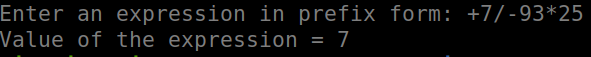
\includegraphics[width=75mm, height=15mm]{pictures/task1_test1.png}} \\ \hline
    2 & \parbox[c]{3cm}{\centering Выражение: +25+/84}
      & 9 & \raisebox{-.5\height}
      {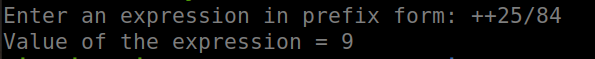
\includegraphics[width=75mm, height=15mm]{pictures/task1_test2.png}} \\ \hline
    3 & \parbox[c]{3cm}{\centering Выражение: *+54+46}
      & 90 & \raisebox{-.5\height}
      {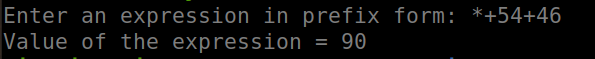
\includegraphics[width=75mm, height=15mm]{pictures/task1_test3.png}} \\ \hline
  \end{tabular}
\end{table}
\subsection{Задача 2}
\subsubsection{Условие задачи}
Разработать функцию(ии) преобразования инфиксной формы
скобочного арифметического выражения в префиксную форму
\subsubsection{Постановка задачи}
Реализовать функцию  преобразования выражения из инфиксной формы в префиксную
и проверить с результатами пункта 1.3.
\subsubsection{Описание подхода решения задачи}
Для этой функции лучше всего использовать алгоритм сортировочной станции для
вывода в виде обратной польской нотации (постфиксной) перевернутого исходного
выражения, а затем переворочивание результата для получения необходимой польской
нотации (префиксной).
\subsubsection{Алгоритм на псевдокоде и описание всех используемых переменных}
Описание переменных: expression - выражение, которое нужно обработать;
 result - результат работы алгоритма;
operators - стек, хранящий в себе все, что не является числами или символами
(т.е. операторы); token - каждый символ в заданном выражении.
\begin{algorithm} % В следующий раз попробую писать как Кормен в Algorithms
  \floatname{algorithm}{Алгоритм}
  \caption{Алгоритм преобразования из инфиксной в префисную форму}
  \label{alg:inf_to_pref}
  \begin{algorithmic}
    \Function{convertFromInfixToPrefix}{expression}
    \State result $\gets$ expression
    \State reverse(result)
    \State reverseParentheses(result) \Comment{Заменяет все '(' на ')' и наоборот}
    \State result $\gets$ convertFromInfixToPostfix(result)
    \State reverse(result)
    \State \Return result
    \EndFunction
  \end{algorithmic}
\end{algorithm}
\begin{algorithm}
  \floatname{algorithm}{Алгоритм}
  \caption{Алгоритм преобразования из инфиксной в постфиксную форму}
  \label{alg:inf_to_postf}
  \begin{algorithmic}
    \Function{convertFromInfixToPostfix}{expression}
    \State Let's operators - stack of the characters
    \State result $\gets$ ""
    \For{every token in a expression}
    \If{token is a number or character}
    \State operators.push(token)
    \ElsIf{token is an operation}
    \While{operators is not empty and precidence of the top operator in operators
    greater than precidence of token and the top operator in operators != '('}
    \State result $\gets$ result + the top operator in operators
    \State operators.pop()
    \EndWhile
    \State operators.push(token)
    \ElsIf{token == '('}
    \State operators.push(token)
    \ElsIf{token == ')'}
    \While{the top operator in operators != '('}
    \State result $\gets$ result + the top operator in operators
    \State operators.pop()
    \If{the top operator == '('}
    \State operators.pop()
    \EndIf
    \EndWhile
    \EndIf
    \EndFor
    \While{operators is not empty}
    \State result $\gets$ result + the top operator in operators
    \State operators.pop()
    \EndWhile
    \State \Return result
    \EndFunction
  \end{algorithmic}
\end{algorithm}
\newpage
\subsubsection{Код программы}
Код алгоритма:
\lstinputlisting[firstline=155, lastline=216]{code/parsing.cpp}
Код main:
\lstinputlisting{code/main2_task.cpp}
\newpage
\subsubsection{Результаты тестирования}
\begin{table}[htpb]
  \centering
  \caption{Тестирование задачи 2}
  \label{tab:task2_test}
  \begin{tabular}{|c|c|c|c|}
    \hline
    \parbox[c]{15mm}{\centering Номер \\ теста} & Входные данные &
    \parbox[m]{3cm}{\centering Ожидаемый \\ результат} &
    \parbox[m]{3cm}{\centering Результат \\ выполнения программы}
    \\ \hline
    1 & \parbox[c]{5cm}{\centering Выражение: (((a+b*c)/d+(x*y-z/k)+m)*n)}
      & \parbox[m]{3cm}{\centering *++/+a*bcd-*xy/zkmn} & \raisebox{-.5\height}
      {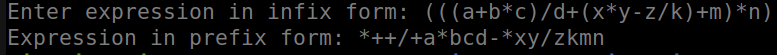
\includegraphics[width=75mm, height=12mm]{pictures/task2_test1.png}} \\ \hline
    2 & \parbox[c]{5cm}{\centering Выражение: a+b/c+d+e-f/m*k}
      & \parbox[m]{3cm}{\centering -+++a/bcde\\*/fmk} & \raisebox{-.5\height}
      {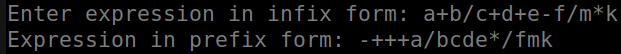
\includegraphics[width=75mm, height=12mm]{pictures/task2_test2.png}} \\ \hline
    3 & \parbox[c]{5cm}{\centering Выражение: (9+3)/2+3*5}
      & \parbox[m]{3cm}{\centering +/+932*35} & \raisebox{-.5\height}
      {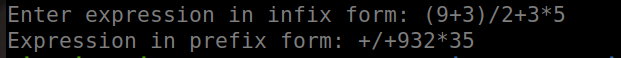
\includegraphics[width=75mm, height=12mm]{pictures/task2_test3.png}} \\ \hline
  \end{tabular}
\end{table}
\subsection{Задача 3}
\subsubsection{Условие задачи}
Дан текст, сформированный по правилу:

<текст>::=<пусто>|<элемент><текст>

<элемент>::=<буква>|(<текст>).

Требуется для каждой пары соответствующих открывающей и
закрывающей скобок вывести номера их позиций в тексте, упорядочив
пары номеров в порядке возрастания номеров позиций:
\begin{enumerate}
  \item закрывающих скобок
  \item открывающих скобок
  \end{enumerate}
Например, для текста А+(45-А(Х)*(В-С)) должно быть выведено:
\begin{enumerate}
  \item 8 10; 12 16; 3 17;
  \item 3 17; 8 10; 12 16;
\end{enumerate}
\subsubsection{Постановка задачи}
Реализовать функцию вывода номеров пар скобок в тексте, упорядочив их порядке
возрастания либо закрывающих, либо открывающих скобок (по выбору пользователя).
\subsubsection{Описание подхода решения задачи}
Для решения задачи нам потребуется стек, в который мы будем класть индексы
встречающихся открывающих ("левых") скобок. При встрече закрывающей ("правой") скобки, мы будем
класть пару текущего индекса правой скобки и индекс на вершине стека в массив из
пар индексов левых и правых скобок. Затем, по решению пользователя, мы сортируем
массив быстрой сортировкой либо по левой, либо по правой скобке.
\subsubsection{Алгоритм на псевдокоде и описание всех используемых переменных}
Описание переменных: expression - выражение, которое нужно обработать;
order - порядок, в котором происходит вывод пар индексов скобок.
Остальные переменные описаны в комментариях псевдокода.
\begin{algorithm}
  \floatname{algorithm}{Алгоритм}
  \caption{Алгоритм функции вывода номеров пар скобок в тексте,
  упорядочив их по выбору пользователя}
  \label{alg:paranthesis_alg}
  \begin{algorithmic}
    \Procedure{outputGroupOfParanthesesByOrder}{expression, order}
    \State Let's left\_par\_ids - stack of integers \Comment стек из индексов левых скобок
    \State Let's v - vector of pairs of two integers \Comment вектор из пар индексов скобок
    \For{i = 0 to the size of expression}
    \If{expression[i] == '('}
    \State left\_par\_ids.push(i+1)
    \ElsIf{expression[i] == ')'}
    \State left\_id $\gets$ the top of left\_par\_ids \Comment индекс левой скобки
    \State left\_par\_ids.pop()
    \State right\_id $\gets$ i + 1 \Comment индекс правой скобки
    \State v.push\_back(pair of left\_id and right\_id)
    \EndIf
    \EndFor
    \If{sort by right paranthesis}
    \State v is sorted by right paranthesis
    \Else \State v is sorted by left paranthesis
    \EndIf
    \For{each element in v}
    \State Print to the screen pair of ids with ';' at the end
    \EndFor
    \State Print end line
    \EndProcedure
  \end{algorithmic}
\end{algorithm}

\subsubsection{Код программы}
Код алгоритма:
\lstinputlisting[firstline=223]{code/parsing.cpp}
Код main:
\lstinputlisting{code/main3_task.cpp}
\subsubsection{Результаты тестирования}
\begin{table}[htpb]
  \centering
  \caption{Тестирование задачи 3}
  \label{tab:task3_test}
  \begin{tabular}{|c|c|c|c|}
    \hline
    \parbox[c]{15mm}{\centering Номер \\ теста} & Входные данные &
    \parbox[m]{3cm}{\centering Ожидаемый \\ результат} &
    \parbox[m]{3cm}{\centering Результат \\ выполнения программы}
    \\ \hline
    1 & \parbox[c]{5cm}{\centering Выражение: А+(45-А(Х)*(В-С)),\\Порядок: 1}
      & \parbox[m]{3cm}{\centering 3 17; 8 10; 12 16; } & \raisebox{-.5\height}
      {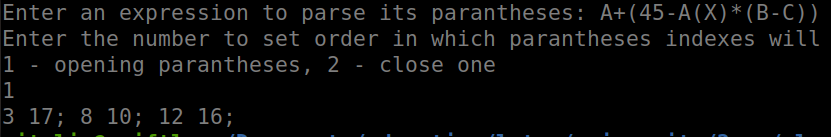
\includegraphics[width=65mm, height=25mm]{pictures/task3_test1.png}} \\ \hline
    2 & \parbox[c]{5cm}{\centering Выражение: А+(45-А(Х)*(В-С)),\\Порядок: 2}
      & \parbox[m]{3cm}{\centering 8 10; 12 16; 3 17} & \raisebox{-.5\height}
      {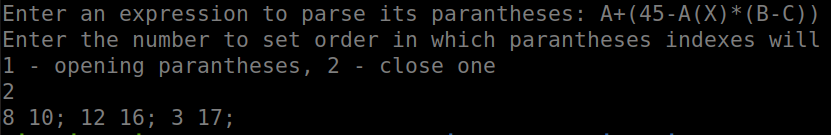
\includegraphics[width=65mm, height=25mm]{pictures/task3_test2.png}} \\ \hline
    3 & \parbox[c]{5cm}{\centering Выражение: (B+(45*C(E))),\\Порядок: 1}
      & \parbox[m]{3cm}{\centering 1 13; 4 12; 9 11; } & \raisebox{-.5\height}
      {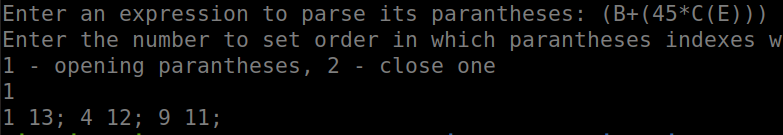
\includegraphics[width=65mm, height=25mm]{pictures/task3_test3.png}} \\ \hline
  \end{tabular}
\end{table}
\newpage
\section*{Выводы}
\addcontentsline{toc}{section}{Выводы}
В ходе практической работы был рассмотрен метод применения стека и очереди при
преобразовании арифметических выражений в постфиксную, префиксную
нотации и вычислении значений выражений; получены знания и навыки по
реализации структуры стек и очередь и функций преобразований выражений.
Также были полученые навыки по написанию алгоритма на псевдокоде.
Каждая функция прошла тестирование успешно, что подтверждает правильную
работу алгоритмов.
\section*{Список информационных источников}
\addcontentsline{toc}{section}{Список информационных источников}
\begin{enumerate}[leftmargin=*]
  \item Thomas H. Cormen, Clifford Stein и другие: Introduction to Algorithms, 3rd Edition.
    Сентябрь 2009. The MIT Press.
  \item N. Wirth: Algorithms and Data Structures. Август 2004.
    \\ https://people.inf.ethz.ch/wirth/AD.pdf.
  \item Shunting-yard algorithm~//~Wikipedia \\~
    [Электронный ресурс]. URL:
    \\ https://en.wikipedia.org/wiki/Shunting-yard\_algorithm
    (Дата обращения: 05.05.2021)
   \item Курс Algorithms, part 2 // Coursera [Электронный ресурс]. URL:
     \\ https://www.coursera.org/learn/algorithms-part2
     (Дата обращения: 05.05.2021)
\end{enumerate}
\end{document}
